\documentclass[12pt]{article}

% Packages
\usepackage[utf8]{inputenc}         % UTF-8 encoding
\usepackage{amsmath}                % Math symbols
\usepackage{graphicx}               % For including images
\usepackage{geometry}               % Page layout
\usepackage{caption}                % Better captions
\usepackage[hidelinks]{hyperref}    % Hyperlinks in the document
\geometry{a4paper, margin=1in}      % Set margins

% Title Page
\title{Informe práctica: \textit{Método de Huckel}}
\author{Nicolás de Pineda Gutiérrez \\[1ex] 
\small Universidad de Sevilla}
\date{}
\begin{document}

\maketitle
\thispagestyle{empty}

\renewcommand{\contentsname}{Contenido}
\newpage
\tableofcontents 

\newpage
\section{Introducción}
El método de orbitales moleculares de Huckel, es un método para aproximar las energías de los orbitales moleculares $\pi$ de sistemas conjugados, como el etileno, butadieno, benzeno, etc. \cite{lowe}

Las energias de los orbitales moleculares $\pi$ de estos sistemas, son particularmente interesantes desde un punto de vista teórico, ya que las propiedades de estos sistemas, como la aromaticidad, la estabilidad, la reactividad, etc., están relacionadas con las energías de los orbitales moleculares $\pi$.

El modelo primero asume que la función de onda de los orbitales $\pi$, es una combinación lineal de los orbitales $p_z$ de los átomos que participan en el sistema $\pi$, ignorando cualquier posible interacción entre los orbitales $\pi$ y los orbitales $\sigma$. Ejemplo, para el etileno:

\[\Psi_\pi = 2c_1\ \phi_{1} + 2c_2\ \phi_{2}\]

Usando el método variacional lineal, con la función de onda anterior: \cite{libretexts}

\[
E_{\text{trial}} = \frac{\langle \Psi | \hat{H} | \Psi \rangle}{\langle \Psi | \Psi \rangle} \geq E_{0}
\]

Expandiendo, y minimizando para los coeficientes, se pueden obtener las ecuaciones seculares, y a partir de estas, el determinante secular. \cite{yates}

\[
\left| \begin{array}{ccc} 
    H_{11}-ES_{11} & \hdots &   H_{1n}-ES_{1n} \\ 
    \vdots & \ddots &   \vdots \\
    H_{n1}-ES_{n1} & \hdots  &   H_{nn}-ES_{nn}
\end{array} \right|
=0
\]

A partir de este determinante, asumimos que el solapamiento de los orbitales $\pi$ es nulo entre sí.
\[S_{ij} = 0 \quad \forall \, i \neq j\]
También tomamos
\[H_{ij} = \alpha \quad \forall \, i = j \]
\[H_{ij} = \beta \quad \forall \, i, j\ enlazados \]
\[H_{ij} = 0 \quad \forall \, i, j\ no\ enlazados \]

Con lo que nos queda el siguiente determinante secular:
\[
\left| \begin{array}{ccc} 
    \alpha-E & \hdots &   \beta\ \acute{o}\ 0 \\ 
    \vdots & \ddots &   \vdots \\
    \beta\ \acute{o}\ 0 & \hdots  &   \alpha-E
\end{array} \right|
=0
\]

Que se puede simplificar, dividiendo todas las columnas por $\beta$, y sustituyendo usando la igualdad $\left(\alpha - E\right)/\beta = x $, para facilitar los cálculos.
Este determinante, se puede expandir para obtener el polinomio secular, cuyas soluciones corresponden a los autovalores, que son las energías de los orbitales moleculares $\pi$. \cite{yates}

Utilizaremos un script de python para montar y resolver el determinante secular de forma programática, además de calcular ciertas propiedades a partir de los resultados.






\newpage
\section{Resolución del Butadieno manualmente}
Para el butadieno, tenemos el determinante secular:
\[
\left| \begin{array}{cccc} 
    \alpha-E & \beta    & 0         & 0         \\
    \beta    & \alpha-E & \beta     & 0         \\
    0        & \beta    & \alpha-E  & \beta     \\
    0        & 0        & \beta     & \alpha-E
\end{array} \right|
=0
\]
Simplificando, dividiendo todo por $\beta$ y sustituyendo $x = \left(\alpha - E\right)/\beta$:
\[
\left| \begin{array}{cccc} 
    x & 1 & 0 & 0 \\
    1 & x & 1 & 0 \\
    0 & 1 & x & 1 \\
    0 & 0 & 1 & x
\end{array} \right|
=0
\]
Y resolviendo:
\[
    x \left| \begin{array}{ccc}
        x & 1 & 0 \\
        1 & x & 1 \\
        0 & 1 & x
    \end{array} \right|
    - 1 \left| \begin{array}{ccc}
        1 & 0 & 0 \\
        1 & x & 1 \\
        0 & 1 & x
    \end{array} \right|
    =0
\]

\[
    x^4 - 3x^2 + 1 = 0
\]
Realizando la sustitución $y = x^2$
\[
    y^2 - 3y + 1 = 0
\]
Usando la formula cuadrática, obtenemos que:
\[
    y = \frac{3 \pm \sqrt{5}}{2}
\]
\[
    x = \pm \sqrt{\frac{3 \pm \sqrt{5}}{2}} = \left(\alpha - E\right)/\beta
\]
Por lo que tenemos que la energía es:
\[
    E = \alpha \pm \beta \sqrt{\frac{3 \pm \sqrt{5}}{2}}
\]


\begin{center}
    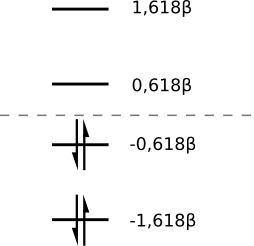
\includegraphics[height=0.24\textwidth]{butadiene_diagram.png}
    \captionof{figure}{Diagrama de orbitales moleculares del butadieno.}
\end{center}

Obtenemos la energía de los orbitales moleculares (Figura 1).






\subsection{Energía total}

Podemos calcular la energía total del sistema, con respecto a los parámetros $\alpha$ y $\beta$, sumando las energías de los orbitales ocupados.

\[E = 2 \left( \alpha + 1.618 \beta \right) + 2 \left( \alpha + 0.618 \beta \right) = 4 \alpha + 4.4721 \beta\]

\subsection{Energía de deslocalización}

La energía de deslocalización es la diferencia entre la energía total del sistema, y la energía que tendría si los enlaces estuvieran localizados.

Si el butadieno tuviera los enlaces localizados, la energía total seria:
\[E_{\text{local}} = 2 (2 \alpha + 2 \beta) = 4 \alpha + 4 \beta\]

Por lo que la energía de deslocalización es:
\[DE = E - E_{\text{local}} = 0.4721 \beta\]

Como $\beta$ es negativo, la energía de deslocalización lo es también, por lo que el sistema es mas estable con los enlaces deslocalizados.

Se suele expresar solo la parte de $\beta$, ya que es la que corresponde a la energia de enlace.  \cite{yates}






\section{Estudio de varios sistemas}

\subsection{Catión, radical y anión alilo}

Energías del catión, radical y anión alilo.
También calculamos la DE (deslocalization energy), que corresponde a restar a la energía total la energía de un sistema sin deslocalización, la BEPE (bonding energy per electron), que es la energía de enlace (x$\beta$) dividida por el número de electrones del sistema y la DEPE (deslocalization energy per electron). \cite{yates}
\begin{center}
\begin{tabular}{|c|c|c|c|}
\hline
    & Catión & Radical & Anión \\
\hline
    $E_{\pi}$ & $2+2.83 \beta$  & $3+2.83 \beta$  & $4+2.83 \beta$ \\
    $BEPE$    & $1.41 \beta$    & $0.943 \beta$   & $0.707 \beta$  \\ 
    $DE$      & $0.83 \beta$    & $0.83 \beta$    & $0.83 \beta$   \\
    $DEPE$    & $0.414 \beta$   & $0.276 \beta$   & $0.207 \beta$  \\ 
\hline
\end{tabular}
\end{center}

\begin{center}
    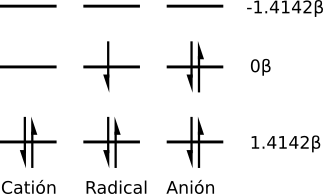
\includegraphics[height=0.25\textwidth]{allyl_diagram.png}
    \captionof{figure}{diagrama de orbitales moleculares del butadieno.}
\end{center}

La energía de deslocalización es igual para los tres casos, pero la energía de enlace por electrón (BEPE), es mayor (más negativa, ya que recordemos que $\beta$ es negativo) para el catión alilo, y menor para el anión alilo, lo que indica que el catión alilo es el mas estable, y el anión alilo el menos estable.

Nota: la comparación de la BEPE calculada es una simplificación grande, ya que no tiene en cuenta que a más electrones, mayor repulsión electrónica, lo que también reduciría la estabilidad, pero el resultado si muestra que no hay ninguna estabilización adicional ocurriendo para el radical o el anión. \cite{yates}

Comparando la DEPE, de nuevo, indica que el catión alilo es el más estabilizado, y el anión alilo el menos estabilizado.






\subsection{Ciclopentadieno, benzeno y cicloheptatrieno}
\begin{center}
    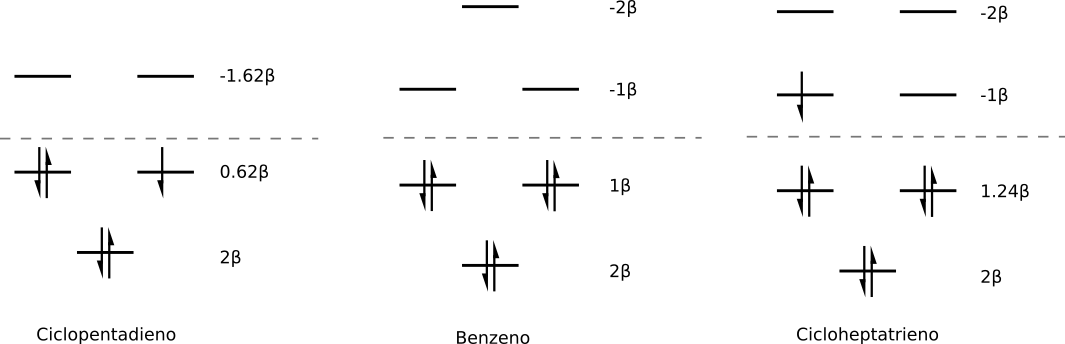
\includegraphics[height=0.25\textwidth]{cycles_diagram.png}
    \captionof{figure}{Diagrama de orbitales moleculares del ciclopentadieno, benzeno y cicloheptatrieno.}
\end{center}

\begin{center}
\begin{tabular}{|c|c|c|c|}
\hline
 &  Ciclopentadieno           & Benzeno         & Cicloheptatrieno \\
\hline
    $E_{\pi}$ & $5+5.85 \beta$  & $6+8  \beta$ & $7+8.54 \beta$ \\
    BEPE      & $1.17   \beta$  & $1.33 \beta$ & $1.22   \beta$ \\ 
    DE        & $1.85   \beta$  & $2    \beta$ & $2.54   \beta$ \\
    DEPE      & $0.37   \beta$  & $0.33 \beta$ & $0.36   \beta$ \\ 
\hline
\end{tabular}
\end{center}

Comparando la BEPE, observamos que el benzeno es el sistema más estable. Esto tiene sentido, ya que el benzeno es aromático. Sin embargo, la energia de deslocalización es mayor para el cicloheptatrieno. Esto se puede explicar debido a que el método, no tiene en cuenta muchos factores importantes, como la repulsión electrónica, o la posición de los átomos.

Las energía HOMO del ciclopentadieno es 0.62$\beta$, y es igual a la del LUMO, por lo que perder un electron haría que se redujese su energía de deslocalización, y ganar un electron haría que aumentase. Esto tiene sentido, ya que el ciclopentadienilo tiende a ganar un electron, convirtiéndose en aromático.

La energía HOMO del benzeno, es 1$\beta$, y la del LUMO -1$\beta$. Esto significa que para el benzeno, tanto perder como ganar un electron, significaría que se redujese su energía de deslocalización, haciéndose menos estable, algo que también tiene sentido, ya que el benzeno es muy estable, no teniendo facilidad para perder o ganar electrones, por su aromaticidad.

Por ultimo, la energía HOMO del cicloheptatrieno, es -1$\beta$, por lo que perder un electrón, haría que aumentase su energía de deslocalización. El tropilio, o catión cicloheptatrienilo, es aromático, algo que va de acuerdo con las energías calculadas.





\subsection{Azuleno}
\begin{center}
    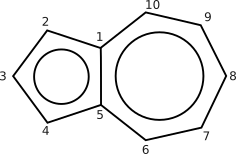
\includegraphics[height=0.25\textwidth]{azulene.png}
    \captionof{figure}{Azuleno numerado}
\end{center}

\begin{center}
\begin{tabular}{|c|c|c|c|}
\hline
     Atom     & Charge density & Net charge   & Free valence \\
\hline
      1       & 1.027          & -0.027       & 1.150 \\
      2       & 1.173          & -0.173       & 0.480 \\
      3       & 1.047          & -0.047       & 0.420 \\
      4       & 1.173          & -0.173       & 0.480 \\
      5       & 1.027          & -0.027       & 0.150 \\
      6       & 0.855          &  0.145       & 0.482 \\
      7       & 0.986          &  0.014       & 0.429 \\
      8       & 0.870          &  0.130       & 0.454 \\
      9       & 0.986          &  0.014       & 0.429 \\
     10       & 0.855          &  0.145       & 0.482 \\
\hline
\end{tabular}
\end{center}

Podemos observar que el anillo de 5 miembros del azuleno tiene una carga neta negativa, y el de 7 miembros una carga neta positiva.

Pensando en el azuleno como un anillo de ciclopentadieno fusionado con una anillo de cicloheptatrieno, podemos explicar esta separación de carga. Los orbitales del anillo de ciclopentadieno, 

Mirando los diagramas de orbitales moleculares del ciclopentadieno, y el cicloheptatrieno, podemos ver que el LUMO del ciclopentadieno, tiene una energía de deslocalización negativa, mientras que el HOMO del cicloheptatrieno, tiene una energía de deslocalización positiva. Por esto, tratando el azuleno como si fueran estos dos anillos unidos, es es coherente asumir que densidad de carga del anillo de 7 miembros, se desplazará hacia el anillo de 5 miembros, reduciendo la energía del sistema.

Esta separación de carga, explica el momento dipolar del azuleno, que es de 1.08D.





\section{Obtención de $\beta$}
\subsection{A partir de energías de deslocalización experimentales}
Podemos calcular la energía de deslocalización de un sistema, en función de $\beta$. Si la representamos frente a la energía de deslocalización experimental, podemos obtener el valor de $\beta$.

\begin{center}
    \begin{tabular}{|c|c|c|}
\hline
& $DE/kcal \cdot mol^{-1} (exp)$ & $DE\ \beta (teor)$ \\
\hline
Benzeno     & 37  & 2     \\
Naftaleno   & 75  & 3.68  \\
Antraceno   & 105 & 5.31  \\
Fenantreno  & 110 & 5.45  \\
\hline
\end{tabular}

\end{center}

Representando la energía de deslocalización experimental frente a la teórica en función de $\beta$
\begin{center}
    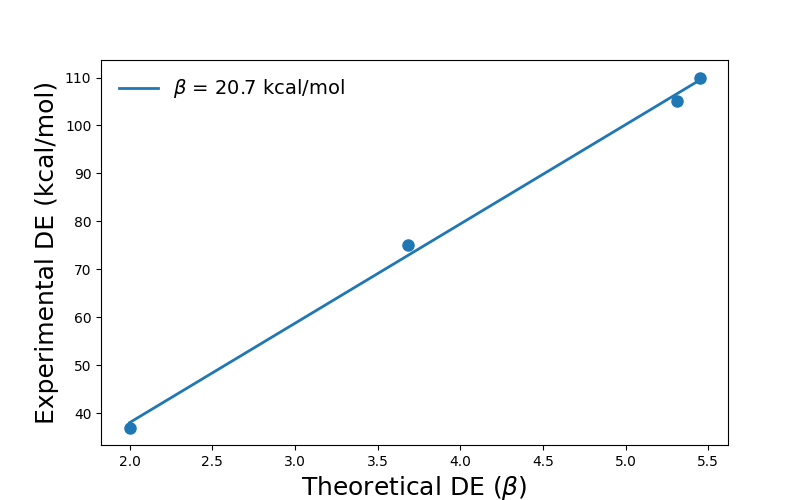
\includegraphics[height=0.37\textwidth]{beta1_plt.png}
    \captionof{figure}{Energía de deslocalización experimental frente a teórica.}
\end{center}
Obtenemos una pendiente de $\beta=20.7kcal/mol$ ($\beta$ es negativo, pero se han representado las energías de deslocalización en valor absoluto).




\subsection{A partir de energías de transición electrónica experimentales}
También podemos obtener $\beta$ a partir de las energías de transición electrónica de un sistema, obtenidas por espectroscopia, y la diferencia de energía HOMO-LUMO teóricas obtenidas por el método de Huckel.
\begin{center}
    \begin{tabular}{|c|c|c|}
\hline
 & $\Delta E_{HOMO-LUMO}\ cm^{-1} (exp)$ & $\Delta E_{HOMO-LUMO}\ \beta (teor)$ \\
\hline
Benzeno    & 50.000  & 2     \\
Naftaleno  & 36.360  & 1.24  \\
Antraceno  & 26.700  & 0.828 \\
Fenantreno & 34.190  & 1.21  \\
Tetraceno  & 21.230  & 0.590 \\
Pireno     & 29.900  & 0.890 \\
\hline
\end{tabular}
\end{center}

Representando la energía de transición electrónica experimental, frente a la teórica:
\begin{center}
    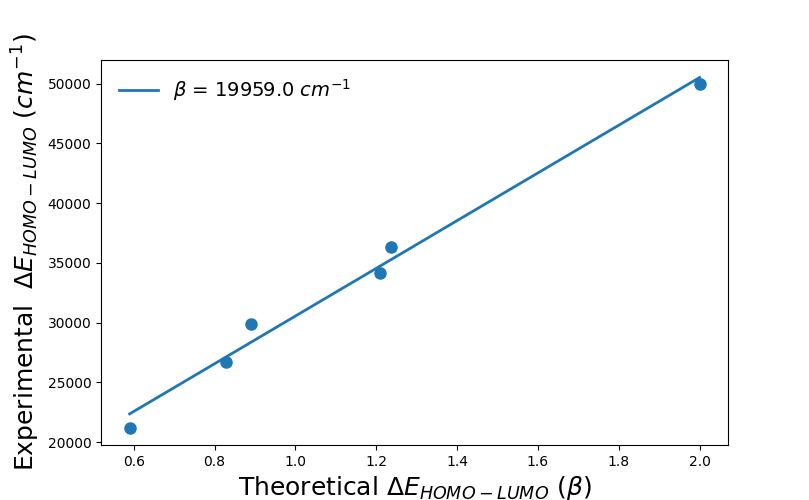
\includegraphics[height=0.37\textwidth]{beta2_plt.png}
    \captionof{figure}{Energía de transición electrónica experimental frente a teórica.}
\end{center}
Obtenemos una pendiente de $\beta=19.959cm^{-1}=57.1kcal/mol$





\subsection{Comparación de los resultados}
El valor obtenido de $\beta$, para la transición electrónica, es bastante mayor al obtenido para la energía de deslocalización, aunque ambos dan una recta lineal.

El método de Huckel es un método simplificado, y no tiene en cuenta muchos factores que pueden afectar a la energía de los orbitales moleculares, como la interacción entre orbitales $\sigma$ y $\pi$, la distancia entre los carbonos, etc.

Estos factores, afectan en distinta medida a la  energía de deslocalización y la energía de transición electrónica. Por ejemplo, la energía de transición electrónica será más sensible a la repulsión electrónica.

Ambas tablas tienen además, una ordenada en el orígen bastante significativa (sobre todo la recta de la energia de transición electrónica), que no tiene una correlación con ningún fenómeno fisico, y se debe puramente a las simplificaciones del método de Huckel.






\subsection{Valor predicho para el criseno}
La diferencia de energía HOMO-LUMO teórica para el criseno, calculada con el método de Huckel es de 1.04$\beta$.
Usando el $\beta$ obtenido a partir de las energías de transición electrónica, obtenemos:

\[
    \Delta E_{HOMO-LUMO}=1.04\beta + 10593cm^{-1}=31350cm^{-1}=89.63kcal/mol
\]

El resultado experimental de 340nm, podemos pasarlo a kcal/mol:
\[
    \frac{1}{340nm} \times \frac{10^9nm}{1m} \times \frac{c\ m}{s} \times h\ Js \times \frac{1kcal}{4184 J} \times N_A = 84.1kcal/mol
\]
Comparándola con el resultado experimental de 340nm, que es igual a 84.1 kcal/mol, se comete un error relativo del 6.6\%. El resultado teórico es una buena aproximación.





\newpage
\begin{thebibliography}{9}


\bibitem{lowe}
John P. Lowe (1993). Quantum Chemistry.

\bibitem{libretexts}
Bethune-Cookman University. (2024). Linear Variational Theory. Available at: \url{https://chem.libretexts.org/Courses/BethuneCookman_University/B-CU%3ACH-331_Physical_Chemistry_I/CH-331_Lectures/Lectures/21%3A_Linear_Variational_Theory}

\bibitem{yates}
Keith Yates (1978). Hückel Molecular Orbital Theory.


\end{thebibliography}

\end{document}
:\While{}
    \State 
\EndWhile
